%Préambule du document :
\documentclass[12pt, a4paper]{book}
%\usepackage[latin1]{inputenc} 

\usepackage{graphicx}
\usepackage{titling}
\usepackage{amssymb} 
\usepackage{minitoc} % chapter's tocs
\usepackage{fancyhdr} % modify the headers
\usepackage{tabularx} % tables not larger than A4
\usepackage[table]{xcolor} %colours inside the tables
\usepackage{float}
\usepackage{multicol} % multiple columns in some sections
\usepackage[inner=2cm,outer=2cm]{geometry} %A4 margins

\usepackage[labelfont=bf]{caption} % for figure captions in minipages

\pagestyle{fancy}
\fancyhead{}
\fancyfoot{}
\fancyhead[RO,LE]{\thepage}
\fancyhead[LO]{\leftmark}
\fancyhead[RE]{\rightmark}

\setcounter{minitocdepth}{1} %we only want sections in minitoc

\pretitle{%
  \begin{center}
  \LARGE
  
\includegraphics[width=12cm]{Logo_software.png}\\[\bigskipamount]
}
\posttitle{\end{center}}

\title{ISE-MeshTools User's guide\\ISE-MeshTools v1.3}



%\titlepicture[width=13cm]{Logo_software.png}
\author{Renaud LEBRUN}
\date{28th february 2016} 


%Corps du document :
\begin{document}

	\dominitoc

	\maketitle
   ISE-MeshTools is a software designed by Renaud Lebrun, from the University of Montpellier. ISE-MeshTools is a 
system for the processing and editing of series of 3D triangular meshes. The system provides a set of tools for editing, 
positioning, deforming, labeling, measuring and rendering sets of 3D meshes. Features include:
\begin{itemize}
\item Retro-deformation for virtual restoration of fossils/deformed specimens;
\item Point and curve primitives for placing the exact type of landmark points you’re interested in
\item Easy to use 3D interface for positioning and manipulating sets of surfaces and landmark primitives
\item Mesh tagging, labeling and coloring (to allow for the creation of anatomy atlases)
\item Mesh scalar computation and colouring (based upon curvature/thickness etc...)
\end{itemize}


\tableofcontents


		 \chapter{Licence}
    
		\minitoc
		
    \section{ISE-MeshTools}
    ISE-MeshTools is Copyright(C) 2013-2016: Renaud LEBRUN, Cécile PELADAN, Stefan SCHLAGER, Jean DUMONCEL. All rights reserved.
This program is free software; you can redistribute it and/or modify it under the terms of the GNU 
General Public License as published by the Free Software Foundation; either version 2 of the License, 
or any later version.\\\\
This program is distributed in the hope that it will be useful, but WITHOUT ANY WARRANTY; without 
even the implied warranty of MERCHANTABILITY or FITNESS FOR A PARTICULAR PURPOSE. See the 
GNU General Public License for more details.

    \section{VTK}
  ISE-MeshTools’ compiled versions contain binary forms of VTK: Copyright (c) 2000-2006 Kitware Inc. 28 
Corporate Drive, Suite 204, Clifton Park, NY, 12065, USA. All rights reserved. Redistribution and use 
in source and binary forms, with or without modification, are permitted provided that the following 
conditions are met:\\
    Redistributions of source code must retain the above copyright notice, this list of conditions and 
the following disclaimer.\\
    Redistributions in binary form must reproduce the above copyright notice, this list of conditions 
and the following disclaimer in the documentation and/or other materials provided with the distribution.//
    Neither the name of Kitware nor the names of any contributors may be used to endorse or promote products derived from this software without specific prior written permission.\\\\
THIS SOFTWARE IS PROVIDED BY THE COPYRIGHT HOLDERS AND CONTRIBUTORS ``AS IS’’ AND ANY 
EXPRESS OR IMPLIED WARRANTIES, INCLUDING, BUT NOT LIMITED TO, THE IMPLIED WARRANTIES 
OF MERCHANTABILITY AND FITNESS FOR A PARTICULAR PURPOSE ARE DISCLAIMED. IN NO EVENT 
SHALL THE AUTHORS OR CONTRIBUTORS BE LIABLE FOR ANY DIRECT, INDIRECT, INCIDENTAL, SPECIAL, 
EXEMPLARY, OR CONSEQUENTIAL DAMAGES (INCLUDING, BUT NOT LIMITED TO, PROCUREMENT OF 
SUBSTITUTE GOODS OR SERVICES; LOSS OF USE, DATA, OR PROFITS; OR BUSINESS INTERRUPTION) 
HOWEVER CAUSED AND ON ANY THEORY OF LIABILITY, WHETHER IN CONTRACT, STRICT LIABILITY, 
OR TORT (INCLUDING NEGLIGENCE OR OTHERWISE) ARISING IN ANY WAY OUT OF THE USE OF THIS 
SOFTWARE, EVEN IF ADVISED OF THE POSSIBILITY OF SUCH DAMAGE.

		  \chapter{F.A.Q.}
  
    \section{How should I cite ISE-MeshTools in scientific publications ?}
    You may  cite ISE-MeshTools with the following reference :\\
		Lebrun, R. ISE-MeshTools, a 3D interactive fossil reconstruction freeware. 
		12th Annual Meeting of EAVP, Torino, Italy; 06/2014.
    \section{Is ISE-MeshTools a geometric morphometrics software ?}
    No. However, you can digitize 3D landmarks on complex 3D surfaces using ISE-MeshTools, which you 
		can use in other software.
		\section{Can I produce/extract 3D meshes out of CT/MRI data using ISE-MeshTools ?}
		No. To extract 3D meshes CT/MRI data sets, you have to use another software. However, you can edit 
		3D Meshes in various ways using ISE-MeshTools.
		\section{Is there a CTRL-Z functionnality around ?}
		No, there is currently no way to cancel any action. So remember to regularly save your work (especially when tagging surfaces), otherwise precious hours of work can be lost in a second.
     \chapter{Interaction modes}
\minitoc  

 \section{Selection modes}
 \subsection{Normal mode}
Press ``
\includegraphics{images/pixmap/Normal_select_mode.png}" to activate this mode.\\
This is the default selection mode. Selected objects (meshes and landmarks) are drawn ``grey". Unselected ``normal" landmarks are red, while ``target" landmarks are yellow. Unselected meshes can be drawn:
\begin{itemize}
\item Using a uniform colour (default modes)
\item According to tag values at each vertex (tag display mode active 
\includegraphics{images/pixmap/Show_Tag_Window.png})
\item	According to scalar values at each vertex (scalar display mode active 
\includegraphics{images/pixmap/show_color_scale.png} )
\end{itemize}



\subsection{Tag mode}
Press ``
\includegraphics{images/pixmap/Tag_select_mode.png}"to activate this mode
This mode is useful when tagging surfaces (as you can only interact with selected objects). Unselected meshes are drawn ``grey".  Unselected ``normal" landmarks are red, while ``target" landmarks are yellow. Selected landmarks are grey, while selected meshes can be drawn:
\begin{itemize}
\item	Using a uniform colour (default modes)
\item According to tag values at each vertex (tag display mode active 
\includegraphics{images/pixmap/Show_Tag_Window.png})
\item	According to scalar values at each vertex (scalar display mode active 
\includegraphics{images/pixmap/show_color_scale.png} )
\section{Interaction modes}
\end{itemize}

\subsection{Camera mode}
  
\includegraphics{images/pixmap/move.png}``Camera mode" is the default interaction mode, and is active on startup. When active, left and middle mouse button drags result in camera rotation/translation, respectively.
\subsection{Object mode}
   
\includegraphics{images/pixmap/move_mode2.png}When active, left and middle mouse button drags result in object rotation/translation, respectively.
\subsection{Landmark mode}
  
\includegraphics{images/pixmap/Landmarks2.png}When active, only landmarks can be selected/unselected via right mouse button drag/click. This mode is useful when editing/placing landmarks. Left and middle mouse button drags result in camera rotation/translation, respectively.

\section{Landmark setting modes}
Landmarks can be set on surfaces by pressing ``L" + left mouse click. 
Two series of conventional landmarks can be set with ISE-MeshTools: ``normal" and ``target" landmarks. Additionally a third landmark series (``flag" landmarks) can be used to label surface structures. 
\subsection{Normal landmark mode}	
Press ``
\includegraphics{images/pixmap/Landmarks4.png}" to activate this mode (this mode is active by default)
\subsection{Target landmark mode}	

Press ``
\includegraphics{images/pixmap/Landmarks6.png}"  to activate this mode
\subsection{Flag landmark mode}	

Press ``
\includegraphics{images/pixmap/Flag01.png}" to activate this mode

	   \chapter{Keyboard and mouse controls}
\minitoc  

 \section{Keyboard and mouse controls}
\rowcolors{2}{}{gray!25}
\begin{tabularx}{\linewidth}{ | c | X | }
 \hline			
   Ctrl+A & Selects all objects \\ \hline				
   Ctrl+D & Unselects all objects \\ \hline				
   L+ left click & Creates a landmark (either ``normal", ``target" or ``flag" landmark). \\ \hline			
L + right click & If a single landmark is selected, its position is
moved. Nothing happens if no landmark is selected
or if more than one landmark are selected \\ \hline			

Left mouse button drag 
& Camera mode : camera rotation.\newline
 Object mode : object rotation.\newline
Landmark mode : camera rotation. \\ \hline			

Ctrl + left mouse button drag 
& Camera mode : object rotation.\newline
 Object mode : camera rotation.\newline
 Landmark mode : object rotation. \\ \hline	
		
Right mouse button drag & Draws a yellow rectangle. Once right button is
released, all objects (surfaces and landmarks)
falling inside the rectangle get selected/unselected,
depending on their initial selection status \\ \hline	
		
Right mouse button click & All objects (surfaces and landmarks) lying at click
location get selected/unselected, depending on
their initial selection status \\ \hline		
	
Middle mouse button roll (roll wheel) & Zoom / unzoom \\ \hline		
	
Middle mouse button drag 
& Camera mode : camera translation\newline
 Object mode : object translation\newline
 Landmark mode : camera translation \\ \hline	
		
Ctrl + middle mouse button drag 
& Camera mode : object translation\newline
Object mode : camera translation\newline
Landmark mode : object translation \\ \hline			

« Del » & All selected objects are deleted \\ \hline			

T + left click & Tag selected surface with active tag value \\ \hline			
 
T + right click & Tag selected surface with ``0" value \\ \hline			

 \end{tabularx}

\section{Additional controls}
Additional controls are available when using ``lasso cut" or ``lasso tag" (lasso mode should be active):\\
\begin{tabularx}{\linewidth}{ | c | X | }
\hline			
Left click & Adds a segment to polygon (segments are drawn yellow) \\ \hline			

Right click & Connects last segment to first segment. If two segments cross each other, lasso action is canceled. Otherwise, the closed polygon is drawn red.\\ \hline			

Middle click or ``C" + right click. & Once the lasso is closed (lasso polygon drawn red
after a right click), all the vertices falling within the clicked region (outside or inside the polygon) are either:\newline
- given the colour corresponding the the active tag (lasso tag)\newline
- inserted into a new objects (lasso cut).\newline 
See lasso cut and lasso tag sections for further information.\\ \hline	
		
T + left click (``lasso tag" only) & Depending on which tag tool is active, if the
lasso is closed (lasso polygon drawn red after a right click) the vertices are painted either :\newline 
- using the pencil\newline 
- using the magic wand\newline 
- using the flood fill\newline 
Tag propagation is restricted within the area defined by the red polygon.\\ \hline		
	
\end{tabularx}


		\chapter{Camera and object GUI main controls}
\minitoc  

 \section{Camera controls}
\subsection{Camera rotation centre}
By default, the camera rotates around the origin of the coordinate system (x=0, y=0, z=0), but by pressing ``
\includegraphics[scale=0.7]{images/pixmap/Move_cam.png}", the camera will revolve around the centre of mass of all opened objects. The latter option is useful when the centre of mass of an object (or of several ones) is far from the origin of the coordinate system. The grid is drawn using different colors depending on the camera rotation centre (see Fig. \ref{grid_color}). The camera centre can also be set at the location of one of the first 10 ``normal" landmarks (see section \ref{camera_centre_at}).

\begin{figure}
  \centering
  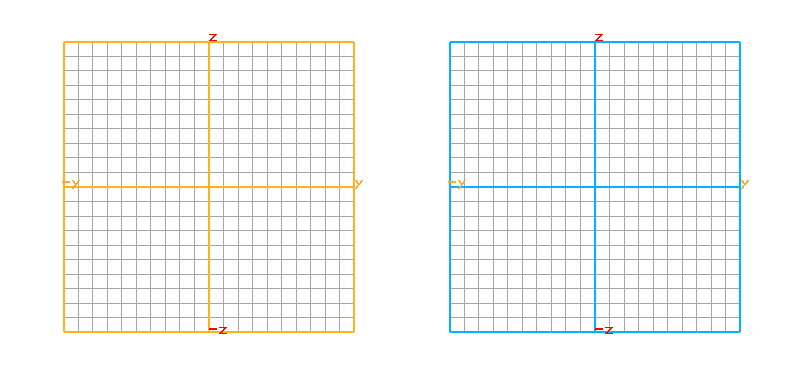
\includegraphics[scale=0.4]{images/GUI/Camera_rotation_centre.png} 
	\caption{Grid display coulour. Left: when the camera revolves around the origin of the coordinate system (x=0, y=0, z=0), the grid is displayed in orange. Right: when the camera revolves around the centre of mass of all opened objects, the grid has a blue layout.}
\label{grid_color}
 
\end{figure}

\subsection{Zoom}
There are three ways to modify the ``zoom" in ISE-MeshTools :


\begin{minipage}{0.7\textwidth}
\begin{itemize}
\item You may use the zoom roller laying in the lower part of the right panel of the main window.
\item	You may open the camera options window (viewing opt. $\rightarrow$  Camera $\rightarrow$ Camera options) and modify manually the ``Zoom" control.
\item	You may set manually the display scale (viewing opt $\rightarrow$ Camera $\rightarrow$ Set 100 pixels in mm)
\item	You may use the middle click mouse roll button (roll the wheel).
\end{itemize}
\end{minipage}    
\begin{minipage}{0.25\textwidth}\centering
  
\includegraphics[scale=0.5]{images/Icons/zoom_01.png}
 \captionof{figure}{Zoom Roll}
 \end{minipage}    


When the option ``Adapt field of view depth" is active in the Rendering options window (Viewing opt.$\rightarrow$General rendering options $\rightarrow$ Depth of field of view panel), changing the zoom value will also modify the depth of the field of view (camera.far value) and the position of the clipping plane (camera.tz value). When the option ``Keep current field of view depth" is active, changing the zoom will not affect the camera.far and camera.tz values.

\subsection{Camera rotation around ``z" viewing axis}

\begin{minipage}{0.7\textwidth}
To do so, you may use the slider lying in the upper part of the right panel of the main window.
\end{minipage}    
\begin{minipage}{0.25\textwidth}\centering
  
\includegraphics[scale=0.5]{images/Icons/Rotation_z.png}
 \captionof{figure}{Camera ``z" rotation slider}
 \end{minipage}    



\subsection{Clipping plane}

\begin{minipage}{0.7\textwidth}
In some cases, you may need to displace the viewing clipping plane. To do so, use
the slider lying centrally in the right panel of the main window.\\
You can also modify the clipping plane manually by editing the ``Tz" control in
the camera options window (viewing opt. $\rightarrow$ Camera $\rightarrow$ Camera options).
The buttons 
\includegraphics[scale=0.7]{images/Icons/clipping_plane3.png} and 
\includegraphics[scale=0.7]{images/Icons/clipping_plane2.png} which lie just underneath the clipping plane slider (and
also in the camera option window) also permit to adjust / readjust the position of
the clipping plane at predefined positions :
\begin{itemize}
\item  
\includegraphics[scale=0.7]{images/Icons/clipping_plane3.png}: the clipping plane is placed at z = 0 (all objects having a z coordinate along
z viewing axis smaller than 0 are hidden).
\item	
\includegraphics[scale=0.7]{images/Icons/clipping_plane2.png} : the clipping plane is replaced at its original value : z= - camera.far / 2. This value permits to
view objects having positive and negative coordinates along z viewing axis.

\end{itemize}
\end{minipage}    
\begin{minipage}{0.25\textwidth}\centering
  
\includegraphics[scale=0.5]{images/Icons/clipping_plane.png}
 \captionof{figure}{Camera clipping plane slider}
 \end{minipage}   




\subsection{Camera orientation}
6 camera positions are predefined :\\

\includegraphics[scale=0.7]{images/pixmap/right2.png} view object from right side \\

\includegraphics[scale=0.7]{images/pixmap/left2.png} view object from left side\\

\includegraphics[scale=0.7]{images/pixmap/right2.png} view object from front side (default camera position)\\

\includegraphics[scale=0.7]{images/pixmap/front2.png} view object from back side\\

\includegraphics[scale=0.7]{images/pixmap/above2.png} view object from above\\

\includegraphics[scale=0.7]{images/pixmap/back2.png} view object from below\\

\subsection{Coordinate system orientation helper}
\begin{minipage}{0.7\textwidth}
Press 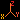
\includegraphics[scale=0.7]{images/pixmap/grid2.png} to show / hide the coordinate system orientation helper lying on the bottom left corner of the main 3D window. By default, the labels are defined
the following way:\\
+z axis : dorsal side\\
-z axis : ventral side\\
+y axis : left side\\
-y axis : right side\\
+x axis : proximal side\\
-x axis : distal side.\\
You may edit these labels depending on your preferences (for instance,
depending on the structure you are working with, you may need to set ``+y" to ``labial", and ``-y" to
``lateral"). To edit orientation labels, click on ``viewing opt. $\rightarrow$ Orientation labels."
\end{minipage}    
\begin{minipage}{0.3\textwidth}\centering
 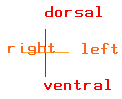
\includegraphics[scale=0.7]{images/GUI/Helper.png}
 \captionof{figure}{Orientation helper}
 \end{minipage}   

\subsection{Grid}
Press 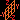
\includegraphics[scale=0.7]{images/pixmap/grid3.png} to show / hide the grid. Default grid size is 1 cm / square. Grid size can be edited manually
(viewing opt. $\rightarrow$ Grid size).
Switching between the 6 camera predefined positions defined above (
\includegraphics[scale=0.7]{images/pixmap/right2.png},
\includegraphics[scale=0.7]{images/pixmap/left2.png},
\includegraphics[scale=0.7]{images/pixmap/right2.png}, 
\includegraphics[scale=0.7]{images/pixmap/front2.png}, 
\includegraphics[scale=0.7]{images/pixmap/above2.png} and 
\includegraphics[scale=0.7]{images/pixmap/back2.png})will
affect the plane in which the grid is drawn.

\subsection{Lightning}
6 lightning orientations are predefined :\\

\includegraphics[scale=0.7]{images/pixmap/s_right_17.png}light from right viewing side\\

\includegraphics[scale=0.7]{images/pixmap/s_left_17.png}light from left viewing side\\

\includegraphics[scale=0.7]{images/pixmap/s_face_17.png}light from front viewing side\\

\includegraphics[scale=0.7]{images/pixmap/s_back_18.png}light from back viewing side\\

\includegraphics[scale=0.7]{images/pixmap/s_dessus_18.png}light from above\\

\includegraphics[scale=0.7]{images/pixmap/s_dessous_18.png}light from below\\

  \section{Object controls controls}
	As seen earlier, selected objects can be translated and rotated using the mouse left and middle buttons
(in landmark and camera selection modes, you also need to maintain ``CTRL" button pressed
while dragging the mouse to achieve rotation and translation of selected objects). Alternatively, you
may also use the following controls to accomplish rotation and translation of selected objects. Rotation
is performed around the global center of mass of all selected objects.

\subsection{Rotation around and translation along ``z" viewing axis}

\begin{minipage}{0.7\textwidth}
These controls are extremely useful, as there is no way to achieve rotation
around « z » viewing axis or translation along ``z" viewing axis using the
mouse. \\
To do so, use the slider and roller lying in the upper part of the left panel of the
main window.

\end{minipage}    
\begin{minipage}{0.25\textwidth}\centering
  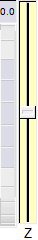
\includegraphics[scale=0.5]{images/Icons/x_rot.png}
 \captionof{figure}{Object ``z" rotation roller and slider}
 \end{minipage}    


\subsection{Rotation around ``x" and translation along ``y" viewing axes}

\begin{minipage}{0.7\textwidth}
To do so, use the slider and roller lying in the lower part of the left panel of the
main window.
\end{minipage}    
\begin{minipage}{0.25\textwidth}\centering
  \includegraphics[scale=0.5]{images/Icons/y_rot.png}
 \captionof{figure}{Object ``x" roller and ``y" slider}
 \end{minipage}   

\subsection{Rotation around ``y" and translation along ``x" viewing axes}


\begin{minipage}{0.5\textwidth}
To do so, use the slider and roller lying in the left part of the bottom panel of the
main window.
\end{minipage}    
\begin{minipage}{0.4\textwidth}\centering
  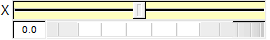
\includegraphics[scale=0.5]{images/Icons/z_rot.png}
 \captionof{figure}{Object ``y" roller and ``z" slider}
 \end{minipage}   


		\chapter{Menu File}
\minitoc  

\section{Open surface}
.stl, .ply, .vtk surfaces can be open via this menu. ISE-MeshTools does not manage textures associated with meshes; still, you can open .obj files, but associated textures will not be loaded. When opening a .ply file containing RGB colours (for instance a file painted manually or automatically with ``MeshLab") or a .vtk file containing RGB scalars, these colours are placed inside the ``RGB" scalars. MeshTools will reinitialize the ``RGB" scalars whenever you change the object's colour or whenever you activate tag display mode or scalar display mode : if these colours are important to you, you may convert them to TAG values in the menu Tags$\rightarrow$Convert RGB colours to tags before changing the object colour or display mode/before changing tags or any colour scale activated.

\section{Save surface}
Selected surfaces can be saved into files. If no surface is selected, the following message appears:\\
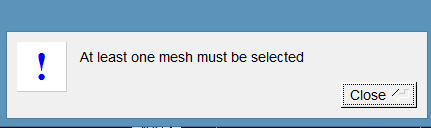
\includegraphics[scale=0.5]{images/File/Save_message.png}
If more than one mesh are selected, the following message shows up:\\
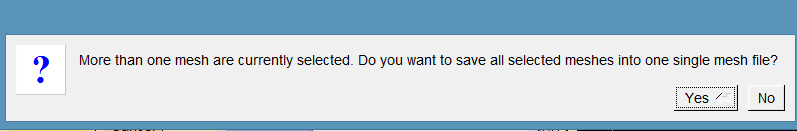
\includegraphics[scale=0.5]{images/File/Save_message2.png}

\subsection{Save .ply}

\begin{minipage}{0.5\textwidth}
Options:
\begin{itemize}
\item File type: you can save .ply data in binary (little or big endian)
or ASCII formats.
\item Position : you can keep object original coordinate system or
save the surface in its current position.
\item Normales : you can chose whether you wish to save normales.
\end{itemize}

\end{minipage}    
\begin{minipage}{0.5\textwidth}\centering
  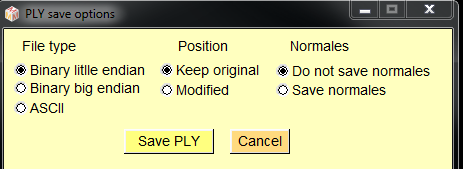
\includegraphics[scale=0.45]{images/File/Save_ply_new.png}
 \captionof{figure}{PLY save options window}
 \end{minipage} 

Note that the ``RGB" scalar (object rendering colour, depending on which rendering mode you
are using) will be saved inside the .ply file. This means that Tag / Scalar / Object colour can be exported and viewed in other software such as MeshLab.


\subsection{Save .stl}

\begin{minipage}{0.5\textwidth}
Options:
\begin{itemize}
\item File type: you can save .stl data in binary (little endian) or
ASCII formats.

\item Position : you can keep object original coordinate system or save the surface in its current position
\end{itemize}

\end{minipage}    
\begin{minipage}{0.5\textwidth}\centering
  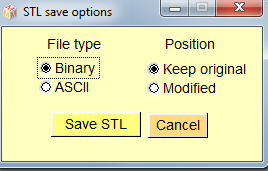
\includegraphics[scale=0.5]{images/File/Save_stl.png}
 \captionof{figure}{STL save options window}
 \end{minipage} 





\subsection{Save .vtk}
\begin{minipage}{0.5\textwidth}
Vtk mesh file format is by far not as widespread as stl or ply
format. However, it is extremely useful as it allows to store
scalar and tag values at each vertex or at each triangle.
Options:
\begin{itemize}
\item File type: you can save .vtk data in binary (little endian) or
ASCII formats.

\item Position : you can keep object original coordinate system
or save the surface in its current position
\end{itemize}
\end{minipage}    
\begin{minipage}{0.5\textwidth}\centering
  \includegraphics[scale=0.5]{images/File/Save_vtk.png}
 \captionof{figure}{VTK save options window}
 \end{minipage} 
\noindent
Note that the ``RGB" scalar (object rendering colour, depending on which rendering mode you are
using) will be saved inside the .vtk file.
\subsection{Save .obj}

\begin{minipage}{0.5\textwidth}
ISE-MeshTools does not manage textures associated with
meshes. Still, you can save meshes in .obj format, but
textures will not be saved.
Options:
\begin{itemize}
\item Position : you can keep object original coordinate system
or save the surface in its current position
\end{itemize}
\end{minipage}    
\begin{minipage}{0.5\textwidth}\centering
  \includegraphics[scale=0.5]{images/File/Save_obj.png}
 \captionof{figure}{OBJ save options window}
 \end{minipage} 


\section{Position}
In ISE-MeshTools, mesh position consists in two
4*4 square matrices: one matrix is used as the
aspect matrix (by default the identity matrix),
and the other one as the position matrix. These
matrices can be opened and saved in ``.pos"
format (see Fig. \ref{position_file}).


\begin{figure}
  \centering
  \includegraphics[scale=0.5]{images/File/Position_file.png}
 \caption{Example of .pos position file. The first 4 lines correspond
to the aspect matrix, and the 4 last lines to the position matrix.}
\label{position_file}
\end{figure}
 



\subsection{Load position}
If no surface is selected, the following message
appears:\\
\includegraphics[scale=0.5]{images/File/open_position1.png}
\\
If more than one mesh are selected, the following message shows up :\\
\includegraphics[scale=0.5]{images/File/open_position2.png}

\subsection{Load transposed position}
This option may be useful in the following case:
\begin{itemize}
\item Let us suppose that you did modify the position of a given surface and saved its position
\item Then you have saved the surface in its current modified position (that is : the original position of the
surface is lost).
\end{itemize}

For some reason, you may need to open the surface in its original position. To do so, you may apply this option (apply transposed position matrix to the modified surface).
Note : this option only works if the aspect matrix was not modified.

\subsection{Save position}
Mesh aspect and position matrices can be saved in ``.pos" format. If no surface is selected, the
following message appears:\\
\includegraphics[scale=0.5]{images/File/save_pos1.png}
\\
If more than one mesh are selected, the following message shows up:\\
\includegraphics[scale=0.5]{images/File/save_pos2png.png}

\subsection{Edit manually aspect and position matrices}
There are two ways to access the object matrix editor :
\begin{itemize}

\item Either select one surface and click on ``\includegraphics[scale=0.7]{images/pixmap/mat.png}"(edit first selected object position and aspect matrices).
\item Or select one surface and click on ``edit selected surfaces$\rightarrow$Rendering modifications$\rightarrow$ edit first
selected object position and aspect matrices".
\end{itemize}



This opens the ``Object Matrix" window, in which the aspect and position matrices can be edited. See ``Edit selected surfaces" section \ref{edit_mat_section} (Rendering modifications$\rightarrow$ edit first selected object position and aspect matrices) for further information.


\section{Project}




When working with multiple surface objects,
loading surfaces and associated positions one
by one becomes fastidious. You may open and
save series of meshes and associated position
matrices using this menu.
``project" files (.ntw) files are organized the
following way (see Fig. \ref{project_file}):
- Name of surface 1 file\\
- Name of position 1 file associated to surface 1\\
- Surface 1 RGB colour and transparency\\
- Name of surface 2 file\\
- Name of position 2 file associated to surface 2\\
- Surface 2 RGB colour and transparency (etc...)\\
 


Surface files can be of the following types : .stl, .vtk, .ply and .obj\\
``.ntw" files can be constructed manually, providing that the refered surface and position files exist.



\begin{figure}
  \centering  
 \includegraphics[scale=0.7]{images/File/Ntw.png}
 \captionof{figure}{Example of project .ntw file}
\label{project_file}
\end{figure}

\subsection{Open project}
Loads a .ntw file

\subsection{Save project}
Saves a .ntw file implicating all selected surfaces. Though ISE-MeshTools can open .ntw files
implicating .stl, .ply and .obj surfaces, when saving a .ntw project, surface files will be saved in .vtk format in order to keep potential tag / scalars associated to each saved surface. Each surface file will be given the name of the original file. Each position file will be given a name which starts with the name of the associated surface and ends with the name of the project. In the .ntw file example shown above, the surface files are 
\begin{itemize}
\item ``Seg-SP07-URM2\_EDJ2.vtk" 
\item ``Seg-SP07-URM2\_OES2.vtk"
\end{itemize}
\noindent and the project name is ``M2\_Sup.ntw". The advantage of naming position files that way is you may construct different .ntw files with different associated surface files using a same set of surfaces.\\
\noindent
\begin{minipage}{0.6\textwidth}
\noindent \noindent Requirement : all selected surfaces saved via this option
need to have distinct names.
Note : When working with ``project" files, you may need at
some point to rename some of the object surfaces. To do so,
select one surface, click on \includegraphics[scale=0.7]{images/pixmap/name.png}: the ``Edit Name" window appears.
Press ok to modify the name of that surface object.
See tutorial ``working with projects" for further information.
\end{minipage}  
 \begin{minipage}{0.4\textwidth}\centering
  \includegraphics[scale=0.5]{images/Icons/edit_name.png}
 \captionof{figure}{Edit name window}
 \end{minipage} 


\section{Landmarks}
As mentioned earlier, landmarks can be set on surfaces by pressing ``L" + left mouse click.\\

Two series ofconventional landmarks can be set : ``normal" and ``target" landmarks. As mentioned earlier, in the ``normal" landmark mode (button \includegraphics[scale=0.7]{images/pixmap/Landmarks4.png} active), pressing ``L" + left mouse click results in
the creation a ``normal" landmark (a red one). In the ``target" landmark mode (button \includegraphics[scale=0.7]{images/pixmap/Landmarks6.png} active),
pressing ``L" + left mouse click will create a ``target" landmark (a yellow one). ``Normal" and ``target" landmarks can be loaded and saved.\\
Selected ``normal"/"target" landmarks can be reordered using the following buttons. Pressing ``\includegraphics[scale=0.7]{images/pixmap/s_dessous_17.png}"
will place the selected landmarks earlier in the ``normal"/"target" landmark list, while pressing ````\includegraphics[scale=0.7]{images/pixmap/s_dessus_17.png}""
will place them one step further, respectively.\\
ISE-MeshTools can manage two types of landmark files: ``.LMK" ``.VER" files.\\ .LMK files contain a series of lines, each line
being constructed the following way (see Fig. \ref{LMK_file}): landmark
name (without space or tab character),
landmark coordinates. Note that each landmark name does not need to be of the form ``landmark"+landmark number. Meanwhile, the name should not hold space or tab
characters.
\\
.VER files contain a series
of lines, each line being
constructed the following
way (see Fig. \ref{VER_file}): landmark name (without space or tab character), landmark coordinates, landmark orientation.

\begin{figure}
  \centering
  \includegraphics[scale=0.7]{images/Landmarks/LMK_file.png}
 \caption{Example of .LMK file}
\label{LMK_file}
\end{figure}

\begin{figure}
  \centering
  \includegraphics[scale=0.7]{images/Landmarks/VER_file.png}
 \caption{Example of .VER file}
\label{VER_file}
\end{figure}


\subsection{Load landmarks}
Landmarks opened using this option will be put in the ``normal" landmark list (red landmarks)
\subsection{Save landmarks}
You may decide whether you wish to save only selected ``normal" landmarks or all selected and
unselected ``normal" landmarks (the red ones).
\subsection{Save target landmarks}

You may decide whether you wish to save only selected ``target" landmarks or all selected and
unselected ``target" landmarks (the red ones).
The ``Landmarks" chapter (chapter \ref{landmark_chapter}) and the tutorial ``working with landmarks" contain further information regarding landmark digitization with ISE-MeshTools

\section{Curves}\label{file_curve_section}
3D Curves are constructed in ISE-MeshTools using 2 series of landmarks : a series of ``normal"
landmarks, and a series of ``target" landmarks of equal sizes. ``Target" landmarks are referred to as
``curve handles", when they are used to construct curves (``Target" landmarks can also be used to
achieve TPS deformation, see later in this documentation). By default, curves are not drawn in the
main 3D window : curves start being drawn when the checkbox ``draw curves" is checked in the menu
``Viewing opt." (\includegraphics[scale=0.7]{images/Landmarks/Draw_curves.png}). Curves are draw green when no landmark/curve handle belonging to
the curve is selected. Curves are drawn red when at least one landmark / curve handle involved in the
curve is selected. Two different cases are considered:
\begin{itemize}

\item Case 1: the numbers of ``normal" and ``handle/target" landmarks differ. In that case, a curve is a series of lines passing through ``normal" landmarks.
\item Case 2: the numbers of ``normal" and ``handle/target" landmarks differ. In that case, a curve is a
series of cubic Bezier curves passing through ``normal" landmarks. For a given set of 2 ``normal"
consecutive landmarks (Ln and Ln+1) and their associated curve ``handles" (Hn and Hn+1), a mirror
image of Hn+1 relative to Ln+1 (H'n+1) is constructed. The Bezier curve involving Ln, Ln+1, Hn and
Hn+1 starts from Ln, going toward Hn, and arrives at Ln+1 coming from the direction of H'n+1.

\end{itemize}


The explicit form of the curve is :
\begin{equation}
B(t) = (1-t)^{3}Ln + 3(1-t)^{3}tHn + 3(1-t)t^{2}H'n+1 +t^{3}Ln+1, t \in[0,1]
\end{equation}
In order to be able to digitize several curves using a given set of normal and target landmarks,
``normal" landmarks curves can be given 4 flags (see section \ref{landmarks_curves_section} ``Landmarks $\rightarrow$ Landmarks
involved into curves" for further details):\\
Flag ``0" : landmark is placed inside the curve (drawn ``red").\\
Flag ``1" : landmark is a curve start (drawn ``green").\\
Flag ``2" : landmark is placed inside the curve, and is a curve ``milestone" (drawn blue) .\\
Flag ``3" : landmark is placed inside the curve, and should be connected to the preceding curve
starting point. When landmark n is flagged that way, landmarkn+1 will be set as a curve starting point.\\
Flag ``2" is used to decompose a given curve into curve segments (see ``export curves as landmark file"). By default, a curve comprises 1 segment\\
Flag ``3" is used to close a curve (by default, curves are open).\\
3D curves are loaded and saved into .CUR files, which contain a series of lines, each line being
constructed the following way: name (without space or tab character), curve ``normal" landmark
coordinates, curve ``handle" coordinates, flag.
In the example shown below, 4 curves are defined :\\
- an open curve starting from landmark 1 and ending at landmark 7\\
- a closed curve involving landmarks 8 to 12\\
- a closed curve involving landmarks 13 to 20\\
- a closed curve involving landmarks 21 to 26\\
These four curves contain only one segment (no curve milestone was set within those 4 curves).
Note that each name does not need to be of the form ``landmark"+ number. Meanwhile, the name
should not hold space or tab characters.
\begin{figure}[t] 
  \centering
  \includegraphics[scale=0.5]{images/Landmarks/CUR_file.png} 
	\caption{Example of .CUR file}
 
\end{figure}

\subsection{Load curves}
This menu allows the user to load a .CUR file.
\subsection{Save curves}
This menu allows the user to save current landmarks and curve handles as a .CUR file. This action is only allowed if the number of ``normal" landmarks and ``target" landmarks is the same. If not, the following message appears:\\
\includegraphics[scale=0.5]{images/Landmarks/Not_identical.png}

\subsection{Export curves as landmark file}
\begin{minipage}{0.55\textwidth}

Curves can be transformed in a series of equidistant
landmarks using this option. The curve decimation window
appears.
Each curve/curve segment is saved as a number of
equidistant landmarks. In the present example, each curve/
curve segment is saved as 20 equidistant landmarks.

\end{minipage}  
 \begin{minipage}{0.45\textwidth}\centering
  \includegraphics[scale=0.5]{images/Landmarks/Export_curves.png}
 \captionof{figure}{Curve decimation window}
 \end{minipage} 

When pressing ``Ok", if the numbers of ``normal" landmarks and ``target" landmarks differ, the
following message appears:\\
\includegraphics[scale=0.5]{images/Landmarks/Can_not_export.png}

\subsection{Save curve infos (length per curve ...)}
\begin{minipage}{0.55\textwidth}

Each curve /curve segment length can be saved as a .txt file
using this option.
The ``Landmarks" chapter (chapter \ref{landmark_chapter}) and the
tutorial ``Working with curves" contain further important
information regarding curve digitization with ISE-MeshTools.

\end{minipage}  
 \begin{minipage}{0.45\textwidth}\centering
  \includegraphics[scale=0.5]{images/Landmarks/Curve_infos.png}
 \captionof{figure}{Example of curve info file}
 \end{minipage} 



\section{Tags and flags}

\begin{minipage}{0.55\textwidth}
- Tag colours and names can be edited interactively by
clicking on \includegraphics[scale=0.7]{images/pixmap/Show_Tag_Window2.png}, which opens the tag window (see the chapter
``Tags" (chapter \ref{tags_chapter}) and the tutorial ``Working with tags" for
further information).\\
- By default, Tags are not visible. To activate/deactivate tag
display, click on \includegraphics[scale=0.7]{images/pixmap/Show_Tag_Window.png}\\
- Using ``Tag display mode" (\includegraphics[scale=0.7]{images/pixmap/Tag_select_mode.png}) is useful when editing
surface tags.\\
25 Tag names and associated colours can be defined in ISEMeshTools.
Tag colours files (.TAG) consist of 25 pairs lines,
each pair being constructed following way :\\
line 2*n: Tag name\\
line 2*n+1: Tag colour and transparency
\end{minipage}  
 \begin{minipage}{0.45\textwidth}\centering
  \includegraphics[scale=0.5]{images/Icons/Tags.png}
 \captionof{figure}{Example of .TAG file}
 \end{minipage} 

\noindent
\begin{minipage}{0.55\textwidth}
Regarding flags, as stated earlier, one series of ``flag landmarks" can be set in ISE-MeshTools (button \includegraphics[scale=0.7]{images/pixmap/Flag01.png} should
be pressed). To edit flag label, length and colour, select one
flag landmark, click on \includegraphics[scale=0.7]{images/pixmap/Flag02.png}. The ``edit flag" window appears.
Pressing ok will update the label, the colour and the
length associated to the selected flag, which in turn will be
unselected. If you wish to edit a second flag, select it and press ``Refresh". The current colour, length
and label of the newly selected flag will appear in the edit flag window.
\end{minipage}  
 \begin{minipage}{0.45\textwidth}\centering
  \includegraphics[scale=0.5]{images/Flags/Edit1flag.png}
 \captionof{figure}{Edit Flag window}
 \end{minipage} 
\noindent
Flags are saved using the .FLG file format, which consists of n pairs of lines constructed the following way :\\
line 2*n: Flag name\\
line 2*n+1: Flag coordinates, flag orientation, flag length and colour.

\subsection{Load tag colours and labels}
Select a .TAG file using this menu $\rightarrow$ Then open the tag window (\includegraphics[scale=0.7]{images/pixmap/Show_Tag_Window2.png}) : Tag labels, colours and
transparencies should have been updated.
\subsection{Save tag colours and labels}
This option saves the current state of tag labels, colours and transparencies in a .TAG file.

\subsection{Load flags}
Select a .FLG file using this menu

\subsection{Save flags}
This option saves the current flag landmarks into a .FLG file, regardless their selection status.

\section{Save infos (surface area, volume...)}
\noindent
\begin{minipage}{0.55\textwidth}

Surface area, volume, triangle number and
vertex number of selected surface objects can be
saved in a .txt file using this option.
\end{minipage}  
 \begin{minipage}{0.45\textwidth}\centering
  \includegraphics[scale=0.4]{images/File/Infos.png}
 \captionof{figure}{Example of info file}
 \end{minipage} 
\noindent

Note: surface objects should be closed in order to provide a correct estimation of object volume.
\section{Orientation labels}
The coordinate system orientation helper labels can be saved into ``.ORI" files, which are .txt files
containing 6 lines, 1 for each axis.


\subsection{Load orientation labels}
Select a .ORI file using this menu $\rightarrow$ Then open the orientation labels window window (Viewing opt;
Orientation labels) : the 6 orientation labels should have been updated.

\subsection{Save orientation labels}
This option saves the current state of orientation labels in a .ORI file.


		
\end{document} 
